
\begin{figure}[H]
\caption{Lote de tareas ejecutando con FCFS}
\label{fig:ej6}
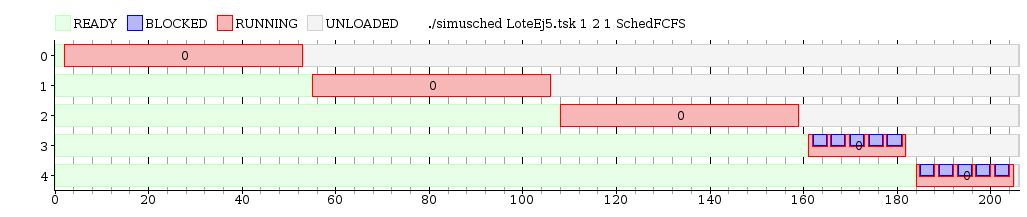
\includegraphics[width=1\textwidth]{imgs/ej6.png}
\end{figure}



\begin{figure}[H]
\begin{center}
  \caption{Datos de las Tareas para FCFS: (en unidades de tiempo)}
\begin{tabular}{| l | c | c | c | c | c | c |}
\hline  
\textbf{Tarea} & \textbf{0} & \textbf{1} & \textbf{2} & \textbf{3} & \textbf{4}  & \textbf{Promedio} \\ \hline
Latencia & 2 & 55 & 108 & 161 & 184 & 102  \\ \hline
Waiting Time & 2 & 55 & 108 & 161 & 184 & 102  \\ \hline
Tiempo Total & 53 & 106 & 159 & 182 & 205 & 141  \\ \hline
\end{tabular}
\end{center}
\end{figure}

\par El scheduler FCFS es el más sencillo de todos: los procesos se ejecutan en orden de llegada, formando una cola. En cambio, los scheduler Round-Robin otorgan un tiempo (quantum) a cada proceso, alternando con desalojos entre cada uno de manera cíclica. Como se ve en la tabla para para este ejemplo, esto produce que el tiempo de respuesta (latencia) usando FCFS sea mayor que utilizando una política Round-Robin. 
\par Con respecto al waiting time y al tiempo total, para este lote de tareas particular, FCFS saca ventaja al otro mecanismo, debido a que en los casos de quantum 2 y 10, el costo de cambios de contexto es muy grande en proporción al resto, mientras que en el de quantum 50, los tiempos se extienden mucho pues las tareas 0 a 2 llevan 51 ciclos de ejecución, provocando una larga espera para ejecutar el exit al final. 
\par Sin embargo, Round-Robin tiene ventajas que no se pueden ver tanto en este ejemplo. Es un mecanismo más equitativo o $"$justo$"$ y, a diferencia de FCFS, optimiza el tiempo de respuesta. Esto suele ser muy útil combinado con prioridades, aunque si se cambia el orden en que se realiza el ciclo puede llegar a a haber inanición, problema que no se presenta usando FCFS.

